\chapter{Filters and Op Amps}
In the last chapter, we learned what op amps are and how we can use two simple rules to analyze their behavior in the context of a given circuit. In the chapter before that, we learned about passive filtering circuits, which selectively attenuate voltage signals based on their frequency content. In this chapter, we will put those concepts together to learn about \textit{active filters}, which not only attenuate signals based on frequency, but also have the potential to \text{amplify} signals in a frequency-dependent way.
\section{Passive Filters with Unity Gain Buffers}
\begin{figure}[h!]
\centering
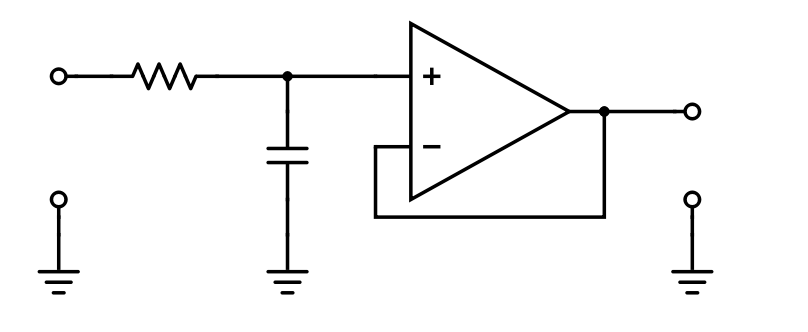
\includegraphics[width=10cm]{figures/bufferedLP.png}
\caption{A passive low-pass filter connected to a unity gain buffer.}
\label{bufferedLP}
\end{figure}

Placing a unity gain buffer after a passive filter as shown in Figure \ref{bufferedLP} mitigates some of the shortcomings of passive filters alone. This circuit acts as a low pass filter, as is clear from the passive low pass filter connected to the non-inverting input. That input is then passed through a unity gain buffer, which can drive any load without its frequency response changing. This is great, because it has the same frequency response as the passive filter alone, and it cannot be loaded down. This configuration could be improved further if we add resistors to the feedback network, thereby providing amplification along with filtering. 
\par
However, this system does have disadvantages; since the filter portion of this circuit is completely separate from the op amp portion of the circuit, the frequency response of the entire system can be affected by passive elements connected to the front end of this circuit. Fortunately, there is a better way.
\section{Active Low-Pass Filter}
\begin{figure}[h!]
\centering
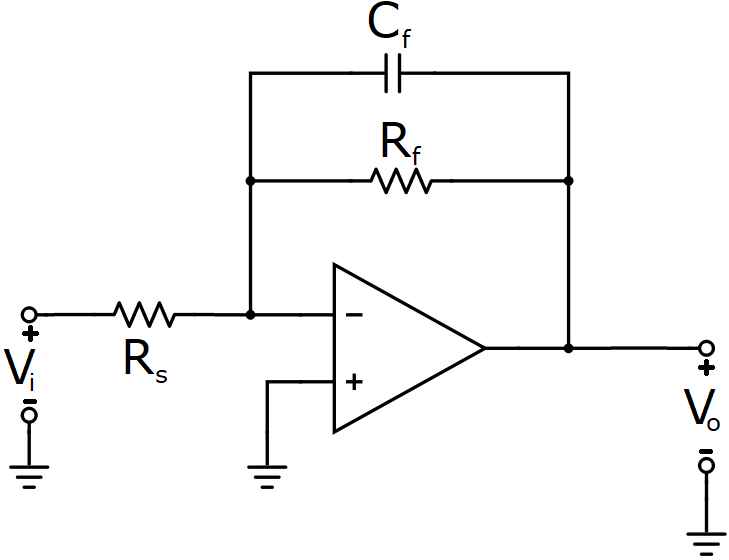
\includegraphics[width=10cm]{figures/activeLP.png}
\caption{An active low-pass filter in an inverting amplifier configuration.}
\label{activeLP}
\end{figure}
Figure \ref{activeLP} shows an inverting amplifier configuration with a resistor and a capacitor in parallel in the feedback network. This is an inverting, active low-pass filter. Let's analyze its voltage gain (which is also its frequency response). First, recall that the voltage gain of the inverting amp is given by $-\frac{Z_f}{Z_s}$. Therefore, we can find the voltage gain of this circuit if we just determine the equivalent impedances of the feedback elements and the source resistance:
$$
Z_f = \frac{1}{\frac{1}{R_f}+j\omega C_f}=\frac{R_f}{1+j\omega R_fC_f}
$$
$$
Z_s = R_s
$$
$$
A_V(j \omega) = -\left(\frac{Z_f}{Z_s}\right) = -\left(\frac{\frac{R_f}{1+j\omega R_fC_f}}{R_s}\right) = -\left(\frac{R_f}{R_s}\right)\cdot\left(\frac{1}{1+j\omega R_fC_f}\right)
$$
\par
This votage gain is the product of two terms; the first term is frequency-independent, and it matches the gain of a purely-resistive inverting amplifier with feedback and source resistors $R_f$ and $R_s$, respectively. The second term matches the frequency response of a passive low-pass filter comprised of elements $R_f$ and $C_f$. This filter is superior to the passive filter and buffer combination of Figure \ref{bufferedLP} because its frequency response is independent of the circuit elements connected either to its input or to its output.
\section{Active High-Pass Filter}
\begin{figure}[h!]
\centering
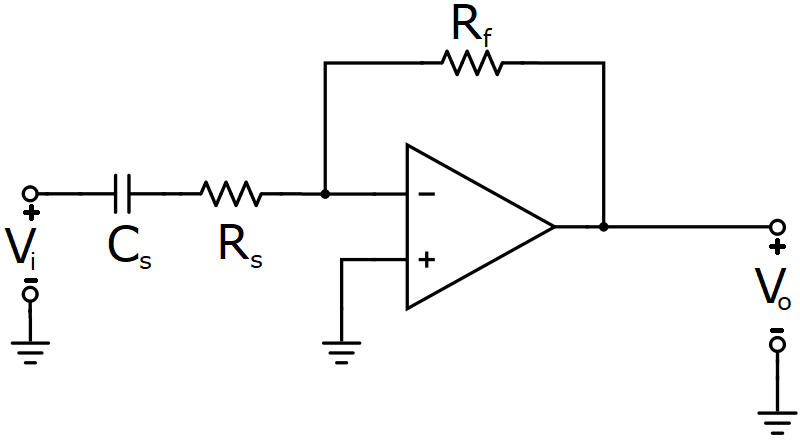
\includegraphics[width=10cm]{figures/activeHP.png}
\caption{An active high-pass filter in an inverting amplifier configuration.}
\label{activeHP}
\end{figure}
In the last section, we replaced the feedback network of an inverting amplifier with a resistor and capacitor in parallel. In this section, we will again start with an inverting amplifier configuration, but we will replace the input network with a resistor and a capacitor in series to produce an inverting, active high-pass filter, as shown in Figure \ref{activeHP}. Let's determine its voltage gain by plugging the input and feedback impedances into the general formula for the inverting amplifier voltage gain:
$$
Z_f = R_f
$$
$$
Z_s = R_s + \frac{1}{j\omega C_s}
$$
$$
A_V(j\omega) = -\left(\frac{R_f}{R_s + \frac{1}{j\omega C_s}}\right) = -\left(\frac{j\omega R_fC_s}{j\omega C_sR_s+1}\right) 
$$
$$
= -\left(\frac{R_f}{R_s}\right)\cdot\left(\frac{j\omega C_s}{j\omega C_s+(1/R_s)}\right)
$$
\par
This voltage gain, like that for the active low-pass filter, is the product of two terms. The first term is the voltage gain for a purely resistive inverting amplifier. The second term is frequency-dependent, and it mirrors the frequency response of a passive high-pass filter. This op amp configuration provides the functionality of a high-pass filter, but with amplification as well. 
\section{Active Band-Pass Filters}
\begin{figure}[h!]
\centering
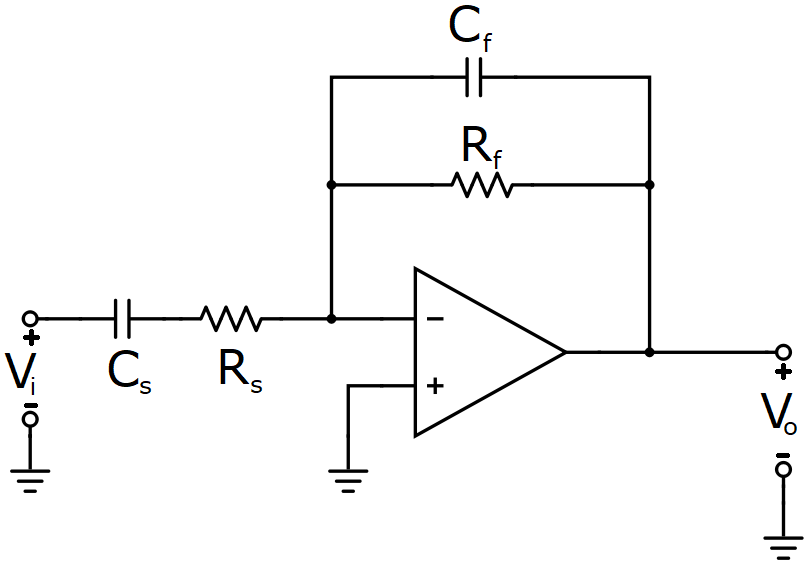
\includegraphics[width=10cm]{figures/activeBP.png}
\caption{An active band-pass filter in an inverting amplifier configuration.}
\label{activeBP}
\end{figure}
I already mentioned some of the negative characteristics of passive filters, but passive band-pass filters have an additional downside in that they require an inductor to function. Inductors tend to be bulky, and that can be a real problem if you are trying to make a circuit as small as possible. The need for inductors is eliminated in the realm of active filters, however.
\par
Let's find the voltage gain for the circuit of Figure \ref{activeBP}. This circuit combines the frequency-dependent feedback and source networks from the active low- and high-pass filters of the previous sections. As we determined before, we can use the impedances of these networks to find the expression for $A_V$ as follows:
$$
Z_f = \frac{R_f}{1+ j\omega R_fC_f}
$$
$$
Z_s = R_s + \frac{1}{j\omega C_s} = \frac{1 + j\omega R_sC_s}{j\omega C_s}
$$
$$
A_V(j\omega) = -\frac{Z_f}{Z_s} = -\frac{j\omega R_fC_s}{(1+ j\omega R_fC_f)(1 + j\omega R_sC_s)}
$$
\par
Even though it looks more complicated, this expression for voltage gain is just the product of a high-pass and a low-pass filter frequency response. The low and high cutoff frequencies are $\omega_{c,low} = \frac{1}{R_fC_f}$ and $\omega_{c,high} = \frac{1}{R_sC_s}$, respectively.
\section{Recap: Op Amp Filter Circuits}
\begin{description}
\item[Active Low-Pass Filter] This filter is described by its voltage gain, which is the product of the voltage gain for a resistive inverting amplifier and the frequency response of a passive low-pass filter:
$$
A_V(j\omega) = -\left(\frac{R_f}{R_s}\right)\cdot\left(\frac{1}{1+j\omega R_fC_f}\right)
$$
\item[Active High-Pass Filter] Like that for the inverting low-pass, the voltage gain for this filter is the product of two terms---the voltage gain for a resistive inverting amplifier, and the frequency response of a passive high-pass filter:
$$
A_V(j\omega) = -\left(\frac{R_f}{R_s}\right)\cdot\left(\frac{j\omega C_s}{j\omega C_s+(1/R_s)}\right)
$$

\item[Active Band-Pass Filter] The voltage gain for this filter is the product of a high-pass and a low-pass frequency response:
$$
A_V(j\omega) = -\frac{j\omega R_fC_s}{(1+ j\omega R_fC_f)(1 + j\omega R_sC_s)}
$$
The low and high cutoff frequencies of this filter are
$$
\omega_{c,low} = \frac{1}{R_fC_f}\textnormal{             and             } \omega_{c,high} = \frac{1}{R_sC_s}
$$
\end{description}